\section{\openFortyTwo と\closeFortyTwo のネットワークの比較}

まず、$\Delta \lambda_{\rm{AB}}$が大きいペアと小さいペアを調べるために、$\Delta \lambda_{\rm{AB}}$ の $\mu \pm 3 \sigma$ よりも外側のペアを抽出した。
図\ref{fig:network_groups_tc_Delta}にドメイン間の$\Delta \lambda_{\rm{AB}}$に着目した図を示す。また、図

\begin{figure}
  \centering
  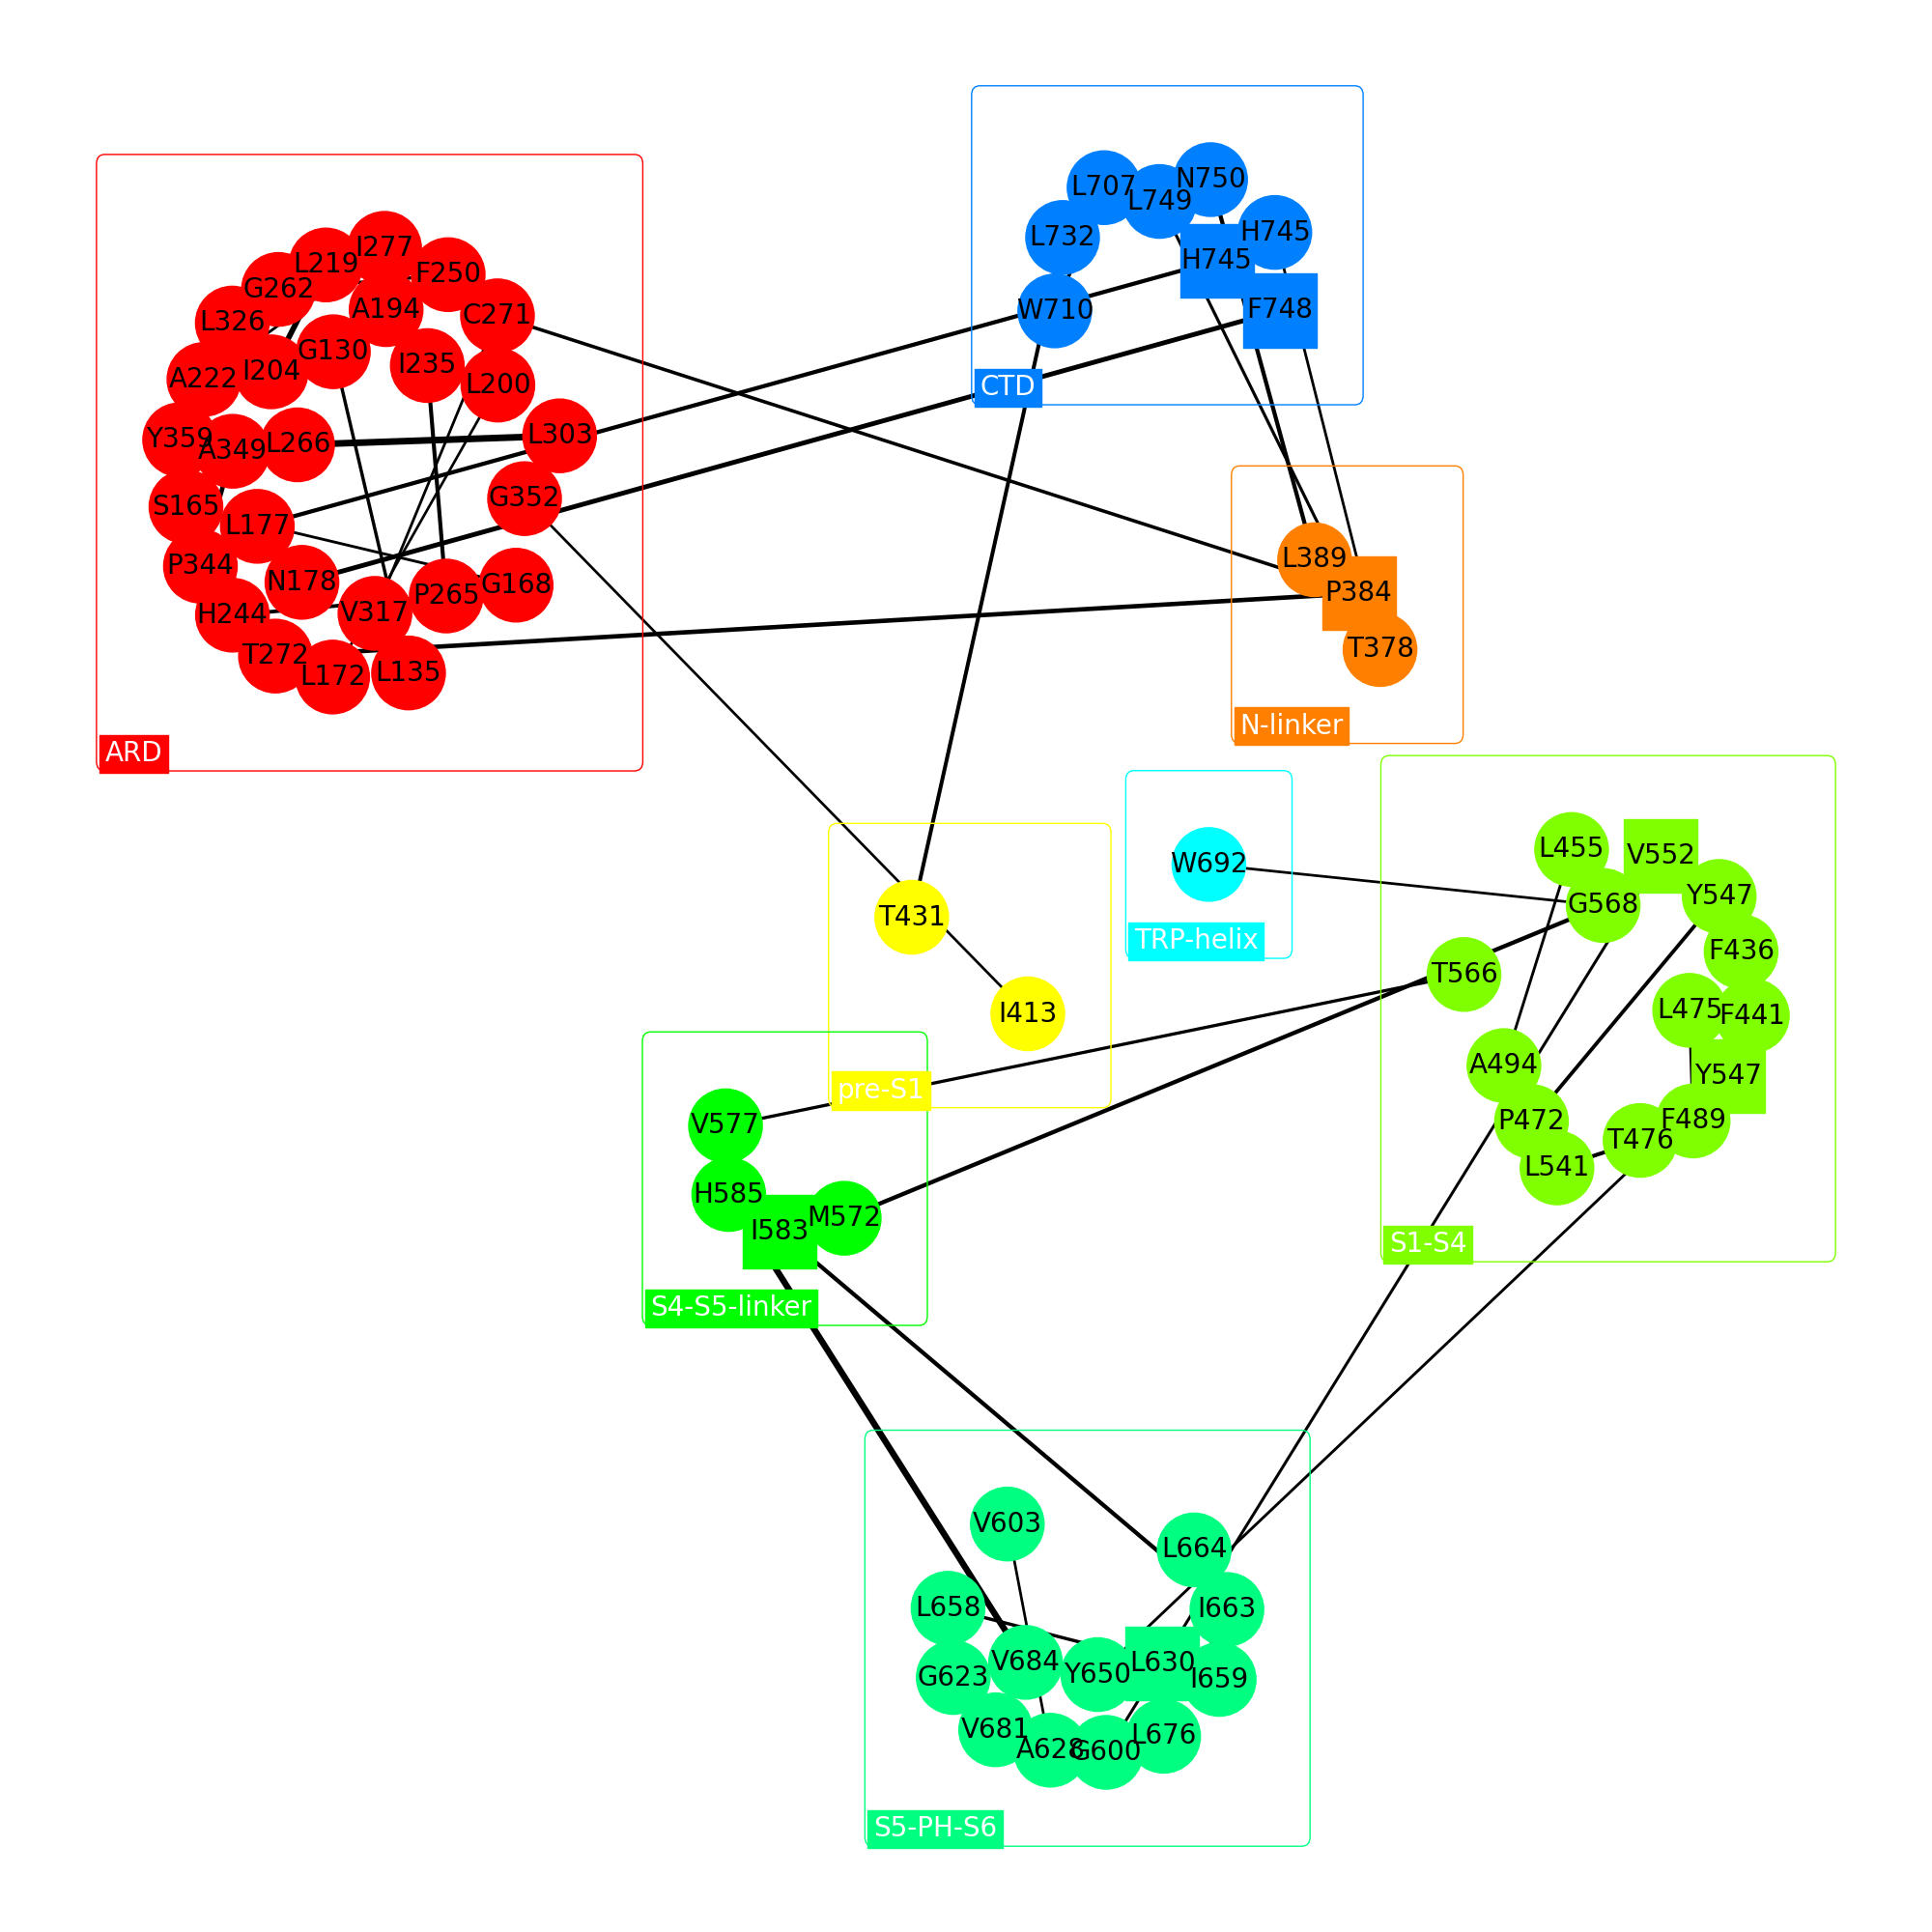
\includegraphics[width=\textwidth]{network_groups_tc_Delta.png}
  \caption{\openFortyTwo と\closeFortyTwo の $\Delta \lambda_{\rm{AB}}$をネットワーク表示した。
            四角形は主鎖Bの残基。ドメインごとに色を分け、N末端側から順にARD、N-linker、pre-S1、S1-S4、S4-S5-linker、S5-PH-S6、TRP-helix、CTDと分けた。
            \autocite{pumroy_structural_2020}}
  \label{fig:network_groups_tc_Delta}
\end{figure}

$\Delta \lambda_{\rm{AB}}$が大きいペアは、

\begin{figure}
  \centering
  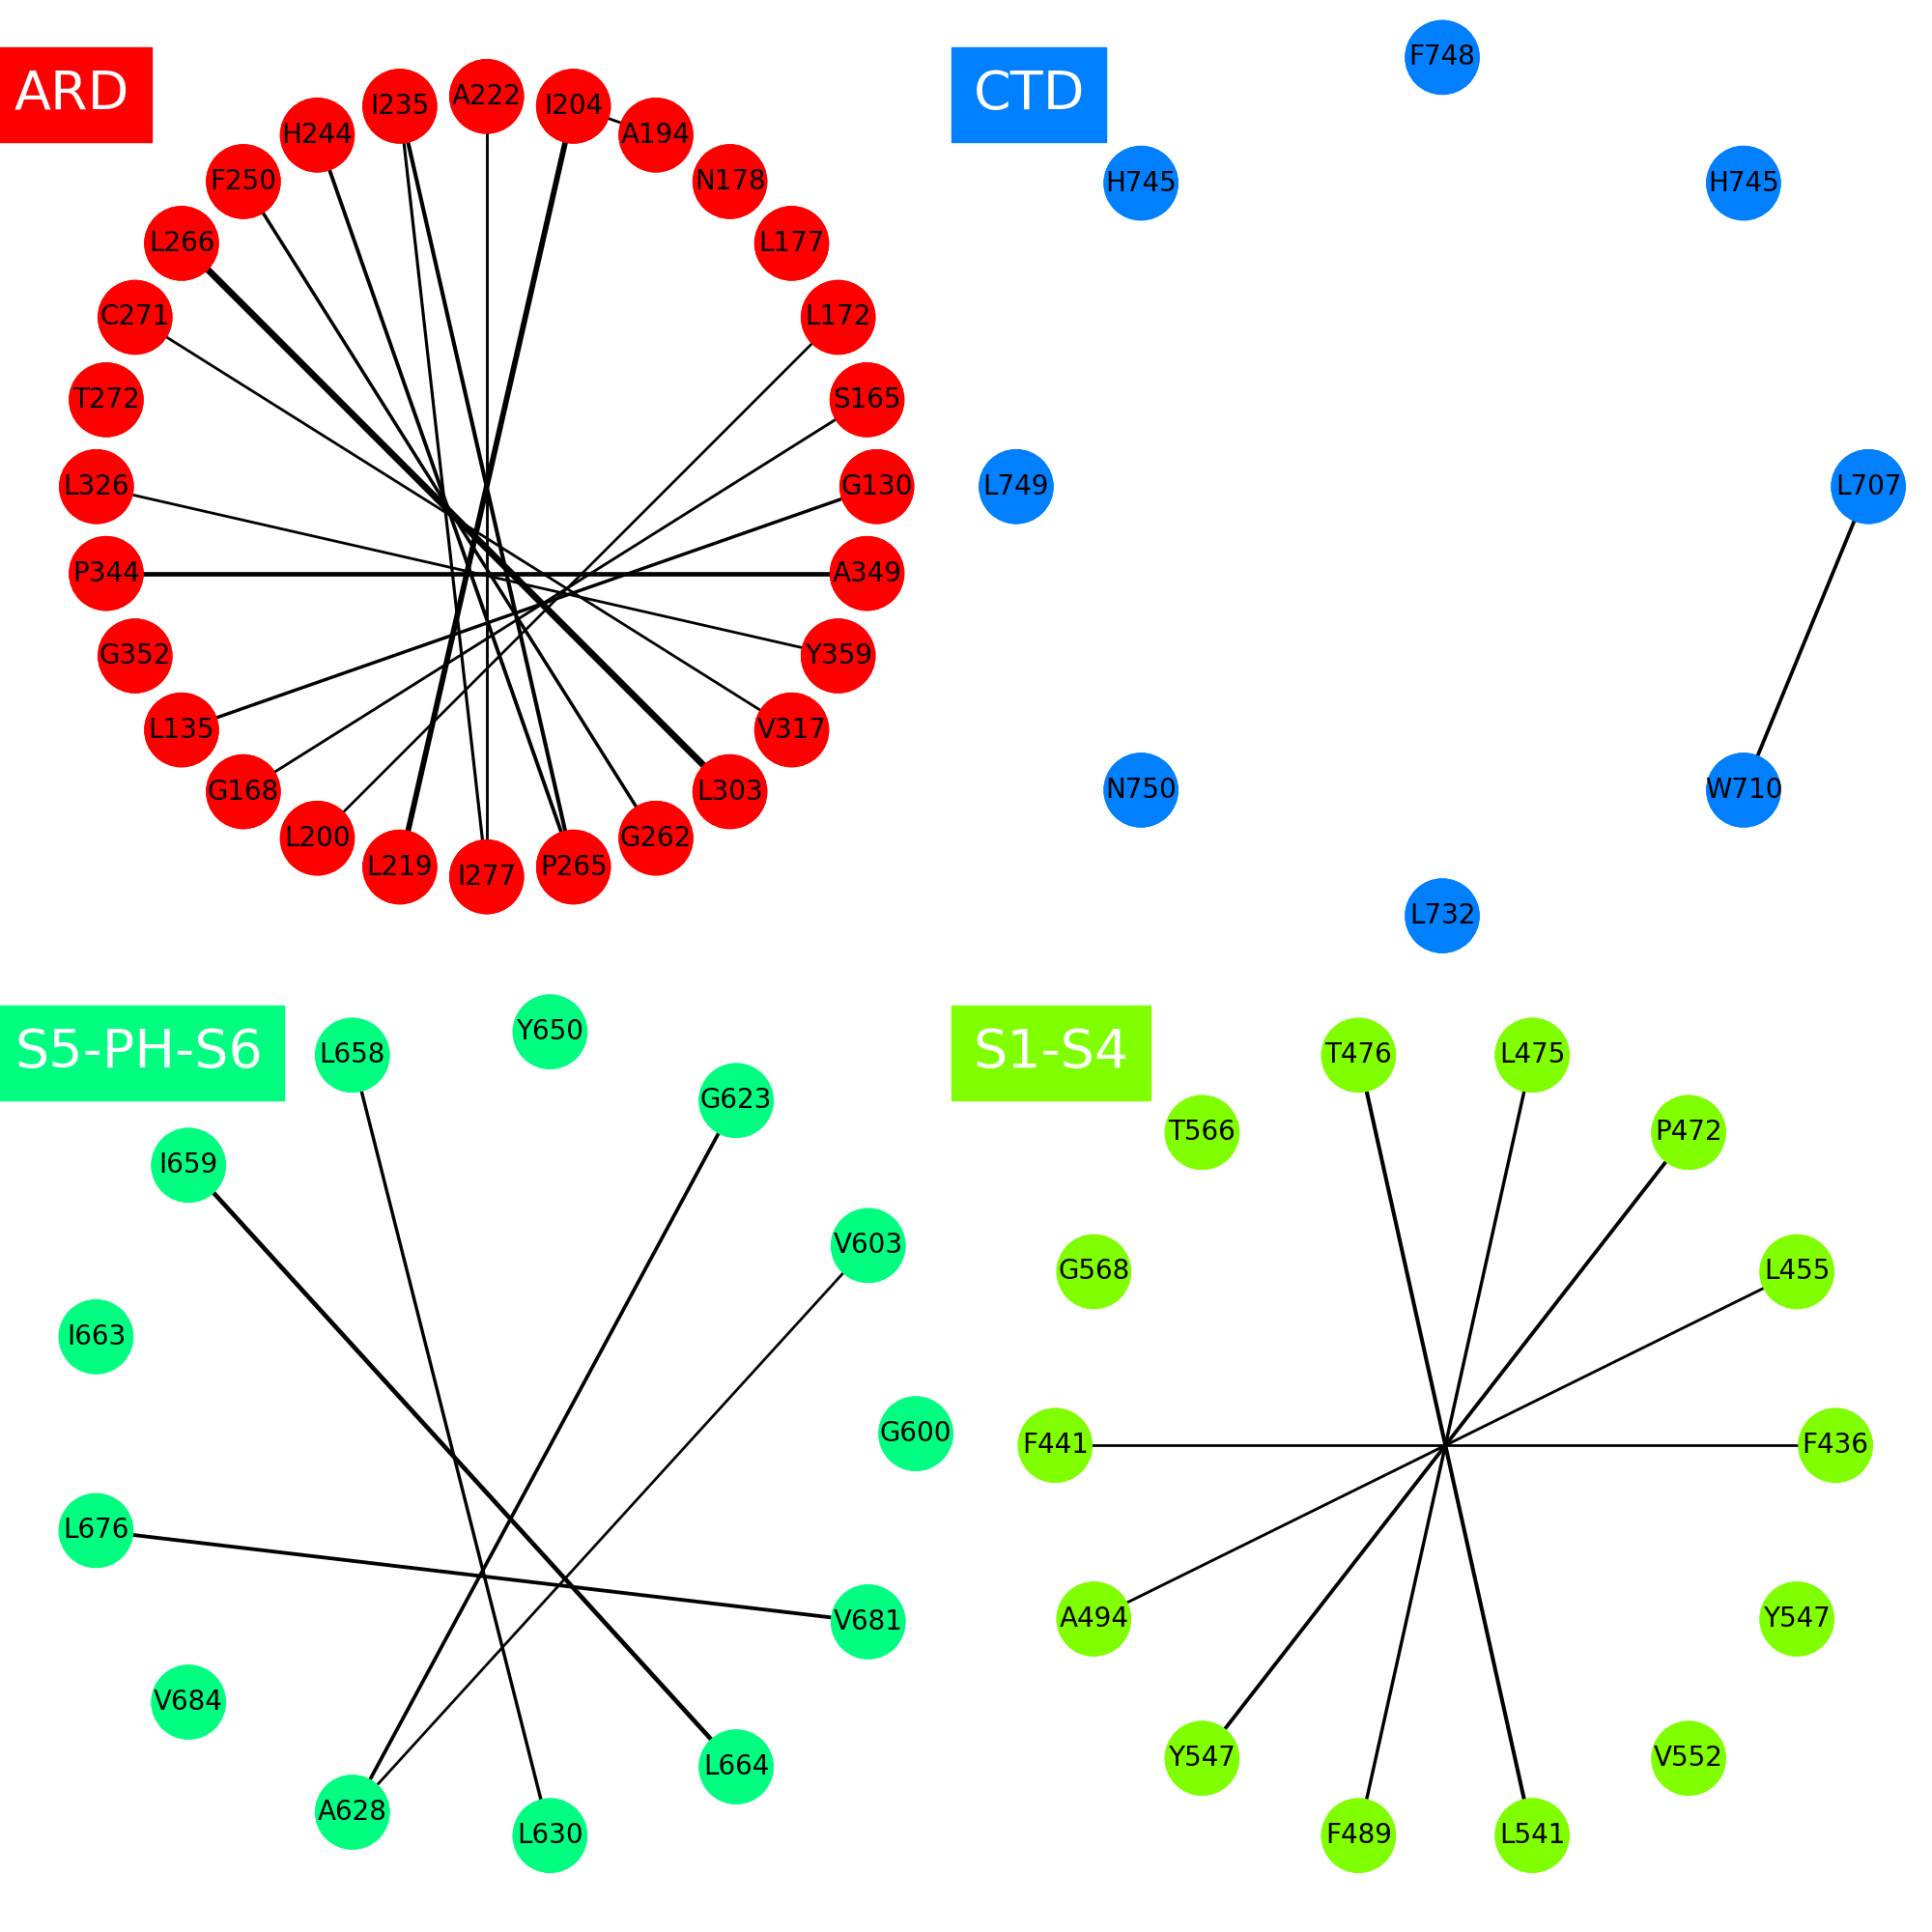
\includegraphics[width=\textwidth]{network_groups_tc_Delta_focus_inside.png}
  \caption{$\Delta \lambda_{\rm{AB}}$が大きいペアのうち、ドメイン内のネットワーク}
  \label{fig:network_groups_tc_Delta_large}
\end{figure}